\documentclass{ximera}

\graphicspath{
  {./}
  {onDifferentDegreesOfSmallness/}
}
\renewcommand{\d}{\mathop{}\!d}

\title{On Relative Growings}

\begin{document}

\begin{abstract}
\end{abstract}
\maketitle

All through the calculus we are dealing with quantities
that are growing, and with rates of growth.
We classify all quantities into two classes: \textit{constants}
and \textit{variables}. Those which we regard as of fixed
value, and call \textit{constants}, we generally denote algebraically
by letters from the beginning of the
alphabet, such as $a$, $b$, or $c$; while those which we
consider as capable of growing, or (as mathematicians
say) of ``varying," we denote by letters from the end
of the alphabet, such as $x$, $y$, $z$, $u$, $v$, $w$, or sometimes $t$.

Moreover, we are usually dealing with more than
one variable at once, and thinking of the way in
which one variable depends on the other: for instance,
we think of the way in which the height reached
by a projectile depends on the time of attaining that
height. Or we are asked to consider a rectangle of
given area, and to enquire how any increase in the
length of it will compel a corresponding decrease in
the breadth of it. Or we think of the way in which
any variation in the slope of a ladder will cause the
height that it reaches, to vary.

Suppose we have got two such variables that depend one on the other. An alteration in one will bring about an alteration in the other, \textit{because} of this
dependence. Let us call one of the variables $x$, and
the other that depends on it $y$.

Suppose we make $x$ to vary, that is to say, we
either alter it or imagine it to be altered, by adding
to it a bit which we call $dx$. We are thus causing $x$
to become $x + dx$. Then, because $x$ has been altered,
$y$ will have altered also, and will have become $y + dy$.
Here the bit $dy$ may be in some cases positive, in
others negative; and it won't (except by a miracle) be
the same size as $dx$.

\begin{image}
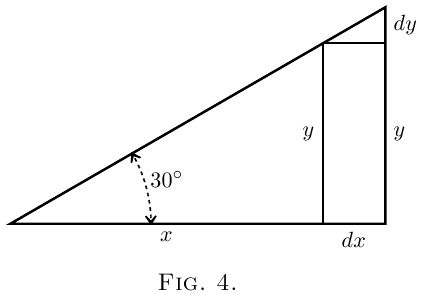
\includegraphics{fig4.png}
\end{image}

% ADD FIGURE 4
\textit{Take two examples.}

(1) Let $x$ and $y$ be respectively the base and the
height of a right-angled triangle 
% ADD hyperlink to Figure 4
of which the slope of the other side is fixed at $30 ^{\circ}$. If we
suppose this triangle to expand and yet keep its
angles the same as at first, then, when the base grows
so as to become $x + dx$, the height becomes $y + dy$.
Here, increasing $x$ results in an increase of $y$. The
little triangle, the height of which is $dy$, and the base
of which is $dx$, is similar to the original triangle; and
it is obvious that the value of the ratio $\dfrac{dy}{dx}$ is the
same as that of the ratio $\dfrac{y}{x}$. As the angle is $30 ^{\circ}$ it
will be seen that here
$$
\frac{dy}{dx} = \frac{1}{1.73}.
$$

(2) Let $x$ represent, in % INSERT HYPERLINK TO FIGURE 5
, the horizontal distance,
from a wall, of the bottom end of a ladder, $AB$,
of fixed length; and let $y$ be the height it
reaches up the wall. Now $y$ clearly depends on $x$.
It is easy to see that, if we pull the bottom end $A$ a
bit further from the wall, the top end $B$ will come
down a little lower. Let us state this in scientific
language. If we increase $x$ to $x + dx$, then $y$ will
become $y - dy$; that is, when $x$ receives a positive
increment, the increment which results to $y$ is
negative.

\begin{image}
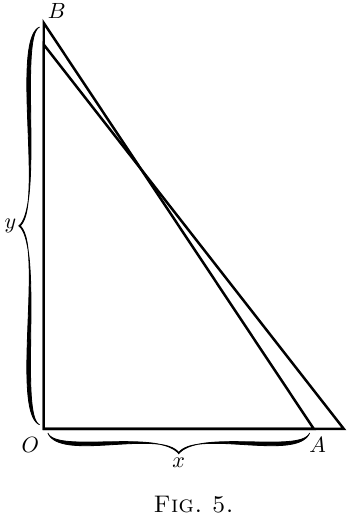
\includegraphics{fig5.png}
\end{image}

Yes, but how much? Suppose the ladder was so
long that when the bottom end $A$ was $19$ inches from
the wall the top end $B$ reached just $15$ feet from the
ground. Now, if you were to pull the bottom end
out $1$ inch more, how much would the top end come
down? Put it all into inches: $x = 19$ inches, $y = 180$
inches. Now the increment of $x$ which we call $dx$,
is $1$ inch: or $x + dx = 20$ inches.

How much will $y$ be diminished? The new height
will be $y - dy$. If we work out the height by Euclid
I. 47, then we shall be able to find how much $dy$ will
be. The length of the ladder is
\[
\sqrt{ (180)^2 + (19)^2 } = 181 \text{ inches}.
\]
Clearly then, the new height, which is $y - dy$, will be
such that
\begin{align*}
(y - dy)^2 &= (181)^2 - (20)^2 = 32761 - 400 = 32361,   \\
y - dy     &= \sqrt{32361} = 179.89 \text{ inches}.
\end{align*}
Now $y$ is $180$, so that $dy$ is $180 - 179.89 = 0.11$ inch.

So we see that making $dx$ an increase of $1$ inch
has resulted in making $dy$ a decrease of $0.11$ inch.

And the ratio of $dy$ to $dx$ may be stated thus:
\[
\frac{dy}{dx} = - \frac{0.11}{1}.
\]

It is also easy to see that (except in one particular
position) $dy$ will be of a different size from $dx$.

Now right through the differential calculus we
are hunting, hunting, hunting for a curious thing, a mere ratio, namely, the proportion which $dy$ bears
to $dx$ when both of them are indefinitely
small.

It should be noted here that we can only find
this ratio $\dfrac{dy}{dx}$ when $y$ and $x$ are related to each
other in some way, so that whenever $x$ varies $y$ does
vary also. For instance, in the first example just
taken, if the base $x$ of the triangle be made longer,
the height $y$ of the triangle becomes greater also,
and in the second example, if the distance $x$ of the
foot of the ladder from the wall be made to increase,
the height $y$ reached by the ladder decreases in a
corresponding manner, slowly at first, but more and
more rapidly as $x$ becomes greater. In these cases
the relation between $x$ and $y$ is perfectly definite,
it can be expressed mathematically, being $\dfrac{y}{x} = \tan 30^{\circ}$
and $x^2 + y^2 = l^2$ (where $l$ is the length of the ladder)
respectively, and $\dfrac{dy}{dx}$ has the meaning we found in
each case.

If, while $x$ is, as before, the distance of the foot
of the ladder from the wall, $y$ is, instead of the
height reached, the horizontal length of the wall, or
the number of bricks in it, or the number of years
since it was built, any change in $x$ would naturally
cause no change whatever in $y$; in this case $\dfrac{dy}{dx}$ has
no meaning whatever, and it is not possible to find an expression for it. Whenever we use differentials
$dx$, $dy$, $dz$, etc., the existence of some kind of
relation between $x$, $y$, $z$, etc., is implied, and this
relation is called a ``function" in $x$, $y$, $z$, etc.; the
two expressions given above, for instance, namely
$\dfrac{y}{x} = \tan 30 ^{\circ}$ and $x^2 + y^2 = l^2$, are functions of $x$ and $y$.
Such expressions contain implicitly (that is, contain
without distinctly showing it) the means of expressing
either $x$ in terms of $y$ or $y$ in terms of $x$, and for
this reason they are called \textit{implicit functions} in
$x$ and $y$; they can be respectively put into the forms
\begin{align*}
y &= x \tan 30^{\circ} \quad\text{or}\quad x = \frac{y}{\tan 30 ^{\circ}} \\
 \text{and}\;
y &= \sqrt{ l^2 - x^2} \quad\text{or}\quad x = \sqrt{ l^2 - y^2}.
\end{align*}

These last expressions state explicitly (that is, distinctly)
the value of $x$ in terms of $y$, or of $y$ in terms
of $x$, and they are for this reason called \textit{explicit
functions} of $x$ or $y$. For example $x^2 + 3 = 2y - 7$ is
an implicit function in $x$ and $y$; it may be written
$y = \dfrac{x^2 + 10}{2}$ (explicit function of $x$) or $x = \sqrt{2y - 10}$
(explicit function of $y$). We see that an explicit
function in $x$, $y$, $z$, etc., is simply something the
value of which changes when $x$, $y$, $z$, etc., are
changing, either one at the time or several together.
Because of this, the value of the explicit function is
called the \textit{dependent variable}, as it depends on the
value of the other variable quantities in the function; these other variables are called the \textit{independent
variables} because their value is not determined from
the value assumed by the function. For example,
if $u = x^2 \sin \theta$, $x$ and $\theta$ are the independent variables,
and $u$ is the dependent variable.

Sometimes the exact relation between several
quantities $x$, $y$, $z$ either is not known or it is not
convenient to state it; it is only known, or convenient
to state, that there is some sort of relation
between these variables, so that one cannot alter
either $x$ or $y$ or $z$ singly without affecting the other
quantities; the existence of a function in $x$, $y$, $z$ is
then indicated by the notation $F(x, y, z)$ (implicit
function) or by $x = F(y, z)$, $y = F(x, z)$ or $z = F(x, y)$
(explicit function). Sometimes the letter $f$ or $\phi$ is used
instead of $F$, so that $y = F(x)$, $y = f(x)$ and $y = \phi(x)$
all mean the same thing, namely, that the value of $y$
depends on the value of $x$ in some way which is
not stated.

We call the ratio $\dfrac{dy}{dx}$ ``the \textit{differential coefficient} of $y$
with respect to $x$.” It is a solemn scientific name
for this very simple thing. But we are not going
to be frightened by solemn names, when the things
themselves are so easy. Instead of being frightened
we will simply pronounce a brief curse on the
stupidity of giving long crack-jaw names; and, having
relieved our minds, will go on to the simple thing
itself, namely the ratio $\dfrac{dy}{dx}$.


In ordinary algebra which you learned at school,
you were always hunting after some unknown
quantity which you called $x$ or $y$; or sometimes
there were two unknown quantities to be hunted
for simultaneously. You have now to learn to go
hunting in a new way; the fox being now neither
$x$ nor $y$. Instead of this you have to hunt for this
curious cub called $\dfrac{dy}{dx}$. The process of finding the
value of $\dfrac{dy}{dx}$ is called ``differentiating.” But, remember,
what is wanted is the value of this ratio when both
$dy$ and $dx$ are themselves indefinitely small. The
true value of the differential coefficient is that to which
it approximates in the limiting case when each of
them is considered as infinitesimally minute.

Let us now learn how to go in quest of $\dfrac{dy}{dx}$.

\begin{center}
\textbf{NOTE TO CHAPTER III.}

\textbf{How to read Differentials.}
\end{center}

It will never do to fall into the schoolboy error of
thinking that $dx$ means $d$ times $x$, for $d$ is not a
factor–it means an ``element of" or ``a bit of"
whatever follows. One reads $dx$ thus: ``dee-eks."

In case the reader has no one to guide him in such
matters it may here be simply said that one reads
differential coefficients in the following way. The
differential coefficient

$\dfrac{dy}{dx}$
is read ``\textit{dee-wy by dee-eks,}" or ``\textit{dee-wy over dee-eks.}"
 So also
$\dfrac{du}{dt}$ is read ``\textit{dee-you by dee-tee.}"

Second differential coefficients will be met with
later on. They are like this: $\dfrac{d^2 y}{dx^2};$
\textit{which is read ``dee-two-wy over dee-eks-squared,"}
and it means that the operation of differentiating $y$
with respect to $x$ has been (or has to be) performed
twice over.

Another way of indicating that a function has been
differentiated is by putting an accent to the symbol of
the function. Thus if $y=F(x)$, which means that $y$
is some unspecified function of $x$, we may
write $F'(x)$ instead of $\dfrac{d\bigl(F(x)\bigr)}{dx}$. Similarly, $F''(x)$
will mean that the original function $F(x)$ has been
differentiated twice over with respect to $x$.

\end{document}